\chapter{El mol y la masa molar}\label{ch:g10:the-mole}

Al final del día, un banco no cuenta sus monedas una a una: las pesa. Si
una moneda tiene una masa de \qty{7.5}{g}, una bolsa de monedas con una
masa de \qty{7.5}{kg} contiene mil monedas, y la balanza ha hecho el
recuento. Los químicos se enfrentan al mismo problema con los \omterm{def:g7:atoms-and-molecules:atom}{átomos},
solo que mucho peor: una cucharada de agua contiene más \omterm{def:g7:atoms-and-molecules:molecule}{moléculas} que
granos de arena hay en todas las playas de una costa. Lo resuelven de la
misma manera, pesando, y la bolsa que usan contiene
\num{602214076000000000000000} entidades. Este capítulo define esa
bolsa, el \omterm{def:g10:the-mole:amount}{mol}, y muestra cómo pasar de una masa medida en una balanza a
un número de \omterm{def:g7:atoms-and-molecules:atom}{átomos} o de \omterm{def:g7:atoms-and-molecules:molecule}{moléculas}.

\begin{recall}
La masa de un \omterm{def:g7:atoms-and-molecules:atom}{átomo} está concentrada en su \omterm{def:g9:inside-the-atom:nucleus}{núcleo}; un \omterm{def:g9:inside-the-atom:proton}{protón} y un
\omterm{def:g9:inside-the-atom:proton}{neutrón} tienen cada uno una masa de unos \qty{1.67e-27}{kg}, así que un
\omterm{def:g7:atoms-and-molecules:atom}{átomo} de \omterm{def:g9:inside-the-atom:atomic-number}{número másico} $A$ tiene una masa de alrededor de
$A \times \qty{1.67e-27}{kg}$. Los números muy grandes y muy pequeños se
escriben en notación científica
(\cref{ch:g9:inside-the-atom}). Una \omterm{def:g7:atoms-and-molecules:formula}{fórmula química} da el número de
\omterm{def:g7:atoms-and-molecules:atom}{átomos} de cada elemento de una \omterm{def:g7:atoms-and-molecules:molecule}{molécula} (\cref{ch:g7:atoms-and-molecules}).
\end{recall}

\begin{omfigure}
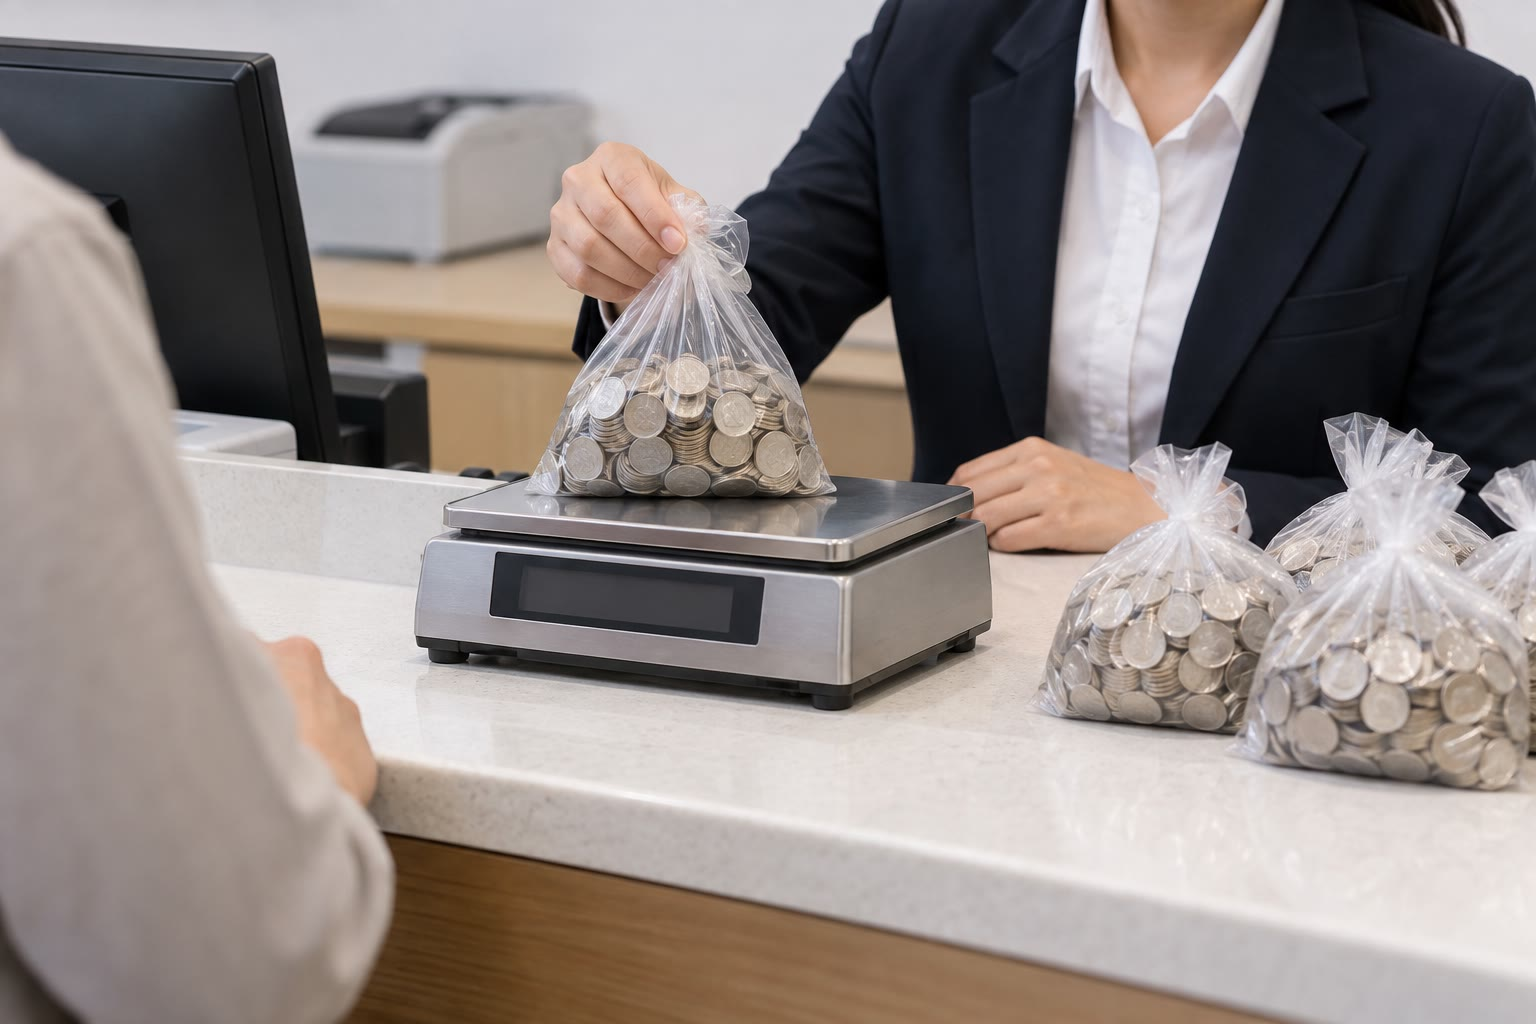
\includegraphics[width=0.55\linewidth]{images/book1/ai/g10-bank-coins.jpg}

{\small Un banco cuenta las monedas pesándolas. Los químicos cuentan los
\omterm{def:g7:atoms-and-molecules:atom}{átomos} de la misma manera.}
\end{omfigure}

\section{Contar pesando}

\begin{example}[Una bolsa de monedas]\label{ex:g10:the-mole:coins}
Una moneda tiene una masa de \qty{7.5}{g}. Una bolsa de estas monedas
tiene una masa de \qty{1.80}{kg}, es decir, \qty{1800}{g}, sin contar la
masa de la propia bolsa. Contiene
\[
  \frac{\qty{1800}{g}}{\qty{7.5}{g}} = 240 \text{ monedas.}
\]
Para contar, el banco divide la masa total entre la masa de una moneda.
\end{example}

\begin{example}[Una cucharada de agua]\label{ex:g10:the-mole:spoon}
Una \omterm{def:g7:atoms-and-molecules:molecule}{molécula} de agua, \ce{H2O}, tiene $2 + 16 = 18$ \omterm{def:g9:inside-the-atom:proton}{nucleones} (los
\omterm{def:g7:atoms-and-molecules:atom}{átomos} de oxígeno~16 y de hidrógeno~1 forman casi toda el agua natural),
así que su masa es de alrededor de
$18 \times \qty{1.67e-27}{kg} = \qty{3.0e-26}{kg}$, o
\qty{3.0e-23}{g}. Una cucharada de \qty{5.0}{g} de agua contiene por
tanto
\[
  \frac{\qty{5.0}{g}}{\qty{3.0e-23}{g}} \approx \num{1.7e23}
  \text{ moléculas.}
\]
La división funciona como con las monedas, pero el resultado es un
número que nadie puede imaginar. Los químicos necesitan un paquete de
\omterm{def:g7:atoms-and-molecules:atom}{átomos} adaptado a las muestras del laboratorio.
\end{example}

\begin{definition}[Cantidad de sustancia y mol]\label{def:g10:the-mole:amount}
% ledger: const:NA
La \emph{cantidad de sustancia}\index{cantidad de sustancia} $n$ de una
muestra cuenta las entidades que contiene (\omterm{def:g7:atoms-and-molecules:atom}{átomos}, \omterm{def:g7:atoms-and-molecules:molecule}{moléculas} o \omterm{def:g9:ions:ion}{iones}, que
se indican cada vez). Su unidad es el \emph{mol}\index{mol}, de símbolo
\si{mol}: un mol contiene exactamente \num{6.02214076e23} entidades.
\end{definition}

\begin{remark}[Una docena, una resma, un mol]\label{rem:g10:the-mole:dozen}
El \omterm{def:g10:the-mole:amount}{mol} es una unidad de recuento, como una docena de huevos (12) o una
resma de papel (500 hojas), solo que muchísimo mayor. ``Dos \omterm{def:g10:the-mole:amount}{moles} de
\omterm{def:g7:atoms-and-molecules:molecule}{moléculas} de agua'' quiere decir
$2 \times \num{6.02214076e23} = \num{1.20e24}$ \omterm{def:g7:atoms-and-molecules:molecule}{moléculas}, igual que ``dos
docenas de huevos'' quiere decir 24 huevos. Hay que decir siempre qué
entidades se cuentan: un \omterm{def:g10:the-mole:amount}{mol} de \emph{\omterm{def:g7:atoms-and-molecules:molecule}{moléculas}} de oxígeno \ce{O2}
contiene dos \omterm{def:g10:the-mole:amount}{moles} de \emph{\omterm{def:g7:atoms-and-molecules:atom}{átomos}} de oxígeno.
\end{remark}

\begin{history}[La hipótesis de Avogadro, 1811]
En 1811, el físico Amedeo Avogadro propuso que volúmenes iguales de
gases distintos, a la misma temperatura y presión, contienen el mismo
número de partículas. Comprendió también que un gas como el oxígeno está
formado por \omterm{def:g7:atoms-and-molecules:molecule}{moléculas} de dos \omterm{def:g7:atoms-and-molecules:atom}{átomos}. Su idea quedó olvidada durante casi
cincuenta años, hasta que Stanislao Cannizzaro la usó en 1860 para
obtener un conjunto coherente de pesos atómicos. La constante que cuenta
las entidades de un \omterm{def:g10:the-mole:amount}{mol} recibió más tarde el nombre de Avogadro; él
nunca conoció su valor.
\end{history}

\begin{omfigure}
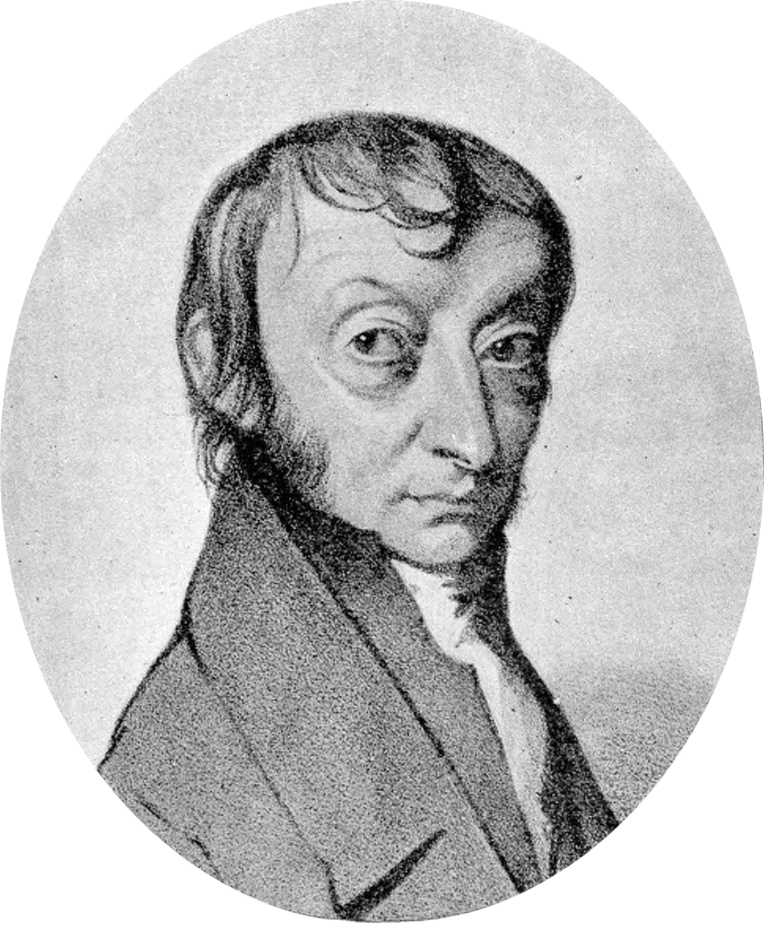
\includegraphics[width=0.26\linewidth]{images/book1/avogadro.jpg}

{\small Amedeo Avogadro (1776--1856).}
\end{omfigure}

\section{La constante de Avogadro}

\begin{definition}[Constante de Avogadro]\label{def:g10:the-mole:avogadro}
% ledger: const:NA
La \emph{constante de Avogadro}\index{constante de Avogadro} $N_A$ es
el número de entidades por \omterm{def:g10:the-mole:amount}{mol}:
\[
  N_A = \qty{6.02214076e23}{mol^{-1}} .
\]
Su valor es exacto, fijado por definición. En los cálculos se redondea a
\qty{6.02e23}{mol^{-1}}.
\end{definition}

\begin{proposition}[Número de entidades y cantidad]\label{prop:g10:the-mole:number}
Una muestra que contiene $N$ entidades contiene la cantidad
\[
  n = \frac{N}{N_A}, \qquad\text{es decir}\qquad N = n \times N_A .
\]
\end{proposition}

\begin{proof}
Cada \omterm{def:g10:the-mole:amount}{mol} contiene $N_A$ entidades, así que $n$ \omterm{def:g10:the-mole:amount}{moles} contienen
$n \times N_A$ entidades; dividiendo entre $N_A$ se obtiene $n$.
\end{proof}

\begin{example}[Moléculas y moles]\label{ex:g10:the-mole:convert}
Una muestra contiene \num{1.5e24} \omterm{def:g7:atoms-and-molecules:molecule}{moléculas} de dióxido de carbono. Su
cantidad de dióxido de carbono es
$n = \num{1.5e24} / \qty{6.02e23}{mol^{-1}} = \qty{2.5}{mol}$.
A la inversa, \qty{0.20}{mol} de hierro contienen
$N = \qty{0.20}{mol} \times \qty{6.02e23}{mol^{-1}} = \num{1.2e23}$
\omterm{def:g7:atoms-and-molecules:atom}{átomos} de hierro.
\end{example}

\begin{remark}[De dónde sale el número]\label{rem:g10:the-mole:origin}
Durante más de cincuenta años, el \omterm{def:g10:the-mole:amount}{mol} se definió como el número de
\omterm{def:g7:atoms-and-molecules:atom}{átomos} que hay en exactamente \qty{12}{g} de carbono~12, y $N_A$ había
que medirlo. Desde 2019 el número mismo está fijado, lo que convierte el
\omterm{def:g10:the-mole:amount}{mol} en un simple recuento. La definición antigua y la nueva coinciden a
mejor que una parte en cien millones, así que doce gramos de carbono~12
siguen conteniendo un \omterm{def:g10:the-mole:amount}{mol} de \omterm{def:g7:atoms-and-molecules:atom}{átomos}, como comprueba la sección
siguiente.
\end{remark}

\section{La masa molar}

\begin{definition}[Masa molar]\label{def:g10:the-mole:molar-mass}
La \emph{masa molar}\index{masa molar} $M$ de una \omterm{def:g6:pure-substances-and-mixtures:species}{especie química} es la
masa de un \omterm{def:g10:the-mole:amount}{mol} de sus entidades, en gramos por \omterm{def:g10:the-mole:amount}{mol} (\si{g/mol}). La
masa molar de un elemento, tomada sobre su \omterm{def:g6:pure-substances-and-mixtures:mixture}{mezcla} natural de \omterm{def:g9:inside-the-atom:isotope}{isótopos},
es su \emph{masa molar atómica}\index{masa molar atomica@masa molar atómica}; figura en la
\omterm{def:g9:periodic-table-first-look:periodic-table}{tabla periódica}.
\end{definition}

\begin{example}[Un mol de átomos de carbono]\label{ex:g10:the-mole:carbon}
% ledger: const:NA, const:u
Un \omterm{def:g7:atoms-and-molecules:atom}{átomo} de carbono~12 tiene una masa de alrededor de
$12 \times \qty{1.67e-27}{kg} = \qty{2.00e-26}{kg}$. Un \omterm{def:g10:the-mole:amount}{mol} de ellos
tiene una masa de
\[
  \qty{2.00e-26}{kg} \times \num{6.02e23} = \qty{1.20e-2}{kg}
  = \qty{12.0}{g}.
\]
El \omterm{def:g10:the-mole:amount}{mol} se ha elegido de modo que la \omterm{def:g10:the-mole:molar-mass}{masa molar} de un \omterm{def:g7:atoms-and-molecules:atom}{átomo}, en gramos
por \omterm{def:g10:the-mole:amount}{mol}, esté cerca de su \omterm{def:g9:inside-the-atom:atomic-number}{número másico}: alrededor de \qty{1}{g/mol}
para el hidrógeno, \qty{12}{g/mol} para el carbono y \qty{16}{g/mol}
para el oxígeno.
\end{example}

\begin{omfigure}
% ledger: aw:H, aw:C, aw:N, aw:O, aw:Na, aw:Mg, aw:Al, aw:Si, aw:S, aw:Cl, aw:K, aw:Ca, aw:Fe, aw:Cu, aw:Zn, aw:Au (rounded to 0.1)
\begin{tabular}{lcr@{\qquad}lcr}
\hline
elemento & símbolo & $M$ (\si{g/mol}) & elemento & símbolo & $M$ (\si{g/mol}) \\
\hline
hidrógeno  & \ce{H}  & 1.0  & silicio   & \ce{Si} & 28.1 \\
carbono    & \ce{C}  & 12.0 & azufre    & \ce{S}  & 32.1 \\
nitrógeno  & \ce{N}  & 14.0 & cloro     & \ce{Cl} & 35.5 \\
oxígeno    & \ce{O}  & 16.0 & potasio   & \ce{K}  & 39.1 \\
sodio      & \ce{Na} & 23.0 & calcio    & \ce{Ca} & 40.1 \\
magnesio   & \ce{Mg} & 24.3 & hierro    & \ce{Fe} & 55.8 \\
aluminio   & \ce{Al} & 27.0 & cobre     & \ce{Cu} & 63.5 \\
           &         &      & oro       & \ce{Au} & 197.0 \\
\hline
\end{tabular}\par\medskip

{\small \omterm{def:g10:the-mole:molar-mass}{Masas molares atómicas} de elementos corrientes, redondeadas a
\qty{0.1}{g/mol}. Son los valores que se usan en este libro.}
\end{omfigure}

\begin{remark}[Por qué el cloro es 35.5]\label{rem:g10:the-mole:chlorine}
% ledger: iso:Cl35, iso:Cl37
El cloro natural es una \omterm{def:g6:pure-substances-and-mixtures:mixture}{mezcla} de dos \omterm{def:g9:inside-the-atom:isotope}{isótopos}: alrededor de tres
cuartas partes de sus \omterm{def:g7:atoms-and-molecules:atom}{átomos} son de cloro~35, y una cuarta parte, de
cloro~37 (\cref{ch:g9:inside-the-atom}). Su \omterm{def:g10:the-mole:molar-mass}{masa molar atómica} es la
media, ponderada por esas proporciones, que queda entre 35 y 37:
\qty{35.5}{g/mol}. Por eso algunas \omterm{def:g10:the-mole:molar-mass}{masas molares atómicas} están lejos
de ser números enteros.
\end{remark}

\begin{proposition}[Masa molar de una molécula]\label{prop:g10:the-mole:sum}
La \omterm{def:g10:the-mole:molar-mass}{masa molar} de una \omterm{def:g7:atoms-and-molecules:molecule}{molécula} es la suma de las \omterm{def:g10:the-mole:molar-mass}{masas molares atómicas}
de todos sus \omterm{def:g7:atoms-and-molecules:atom}{átomos}, cada uno contado tantas veces como aparece en la
fórmula. La misma regla da la \omterm{def:g10:the-mole:molar-mass}{masa molar} de un sólido iónico a partir de
su unidad fórmula.
\end{proposition}

\begin{proof}
Un \omterm{def:g10:the-mole:amount}{mol} de \omterm{def:g7:atoms-and-molecules:molecule}{moléculas} \ce{A_xB_y} contiene $x$ \omterm{def:g10:the-mole:amount}{moles} de \omterm{def:g7:atoms-and-molecules:atom}{átomos} \ce{A} e
$y$ \omterm{def:g10:the-mole:amount}{moles} de \omterm{def:g7:atoms-and-molecules:atom}{átomos} \ce{B}, y nada más; su masa es la suma de las masas
de estos, $x\,M(\ce{A}) + y\,M(\ce{B})$.
\end{proof}

\begin{example}[Tres masas molares]\label{ex:g10:the-mole:three}
% ledger: aw:H, aw:C, aw:O, aw:Na, aw:Cl
\begin{align*}
  M(\ce{H2O}) &= 2 \times 1.0 + 16.0 = \qty{18.0}{g/mol},\\
  M(\ce{NaCl}) &= 23.0 + 35.5 = \qty{58.5}{g/mol},\\
  M(\ce{C12H22O11}) &= 12 \times 12.0 + 22 \times 1.0 + 11 \times 16.0
     = \qty{342.0}{g/mol}.
\end{align*}
La última es la sacarosa, el azúcar de mesa.
\end{example}

\section{De la masa a la cantidad, y al revés}

\begin{proposition}[Masa y cantidad]\label{prop:g10:the-mole:mass}
Una muestra de masa $m$ de una especie de \omterm{def:g10:the-mole:molar-mass}{masa molar} $M$ contiene la
cantidad
\[
  n = \frac{m}{M}, \qquad\text{es decir}\qquad m = n \times M .
\]
Con $m$ en gramos y $M$ en gramos por \omterm{def:g10:the-mole:amount}{mol}, $n$ sale en \omterm{def:g10:the-mole:amount}{moles}.
\end{proposition}

\begin{proof}
Cada \omterm{def:g10:the-mole:amount}{mol} tiene una masa $M$, así que $n$ \omterm{def:g10:the-mole:amount}{moles} tienen una masa
$n \times M$; es el recuento de monedas del banco, con el \omterm{def:g10:the-mole:amount}{mol} como
moneda.
\end{proof}

\begin{method}[De una masa a un número de entidades]\label{met:g10:the-mole:mass-to-number}
\begin{enumerate}
  \item Escribir la fórmula de la especie y calcular su \omterm{def:g10:the-mole:molar-mass}{masa molar} $M$
        con la tabla.
  \item Pasar la masa a gramos si hace falta, y luego $n = m / M$.
  \item Si se pide el número de entidades, $N = n \times N_A$.
  \item Comprobar el orden de magnitud: unos gramos de una \omterm{def:g7:atoms-and-molecules:molecule}{molécula}
        pequeña son del orden de una décima de \omterm{def:g10:the-mole:amount}{mol}, unas $10^{22}$ a
        $10^{23}$ entidades.
\end{enumerate}
\end{method}

\begin{omfigure}
\begin{tikzpicture}[font=\small, box/.style={draw=omDef, very thick,
    fill=omDef!8, rounded corners=3pt, minimum width=2.9cm,
    minimum height=1.1cm, align=center}]
  \node[box] (m) at (0,0) {masa $m$\\[1pt] (\si{g})};
  \node[box] (n) at (5,0) {cantidad $n$\\[1pt] (\si{mol})};
  \node[box] (N) at (10,0) {número $N$\\[1pt] de entidades};
  \draw[-{Stealth[length=7pt]}, thick, omProp] ([yshift=4pt]m.east)
    -- node[above] {$\div M$} ([yshift=4pt]n.west);
  \draw[-{Stealth[length=7pt]}, thick, omProp] ([yshift=-4pt]n.west)
    -- node[below] {$\times M$} ([yshift=-4pt]m.east);
  \draw[-{Stealth[length=7pt]}, thick, omProp] ([yshift=4pt]n.east)
    -- node[above] {$\times N_A$} ([yshift=4pt]N.west);
  \draw[-{Stealth[length=7pt]}, thick, omProp] ([yshift=-4pt]N.west)
    -- node[below] {$\div N_A$} ([yshift=-4pt]n.east);
\end{tikzpicture}

{\small La cantidad $n$ está en el centro: la balanza da $m$, la \omterm{def:g10:the-mole:molar-mass}{masa
molar} lleva a $n$, y la \omterm{def:g10:the-mole:avogadro}{constante de Avogadro} lleva después al número de
entidades.}
\end{omfigure}


\begin{example}[Nueve gramos de agua]\label{ex:g10:the-mole:nine}
% ledger: aw:H, aw:O, const:NA
¿Cuántas \omterm{def:g7:atoms-and-molecules:molecule}{moléculas} hay en \qty{9.0}{g} de agua? $M(\ce{H2O}) =
\qty{18.0}{g/mol}$, así que
\[
  n = \frac{\qty{9.0}{g}}{\qty{18.0}{g/mol}} = \qty{0.50}{mol},
  \qquad
  N = \qty{0.50}{mol} \times \qty{6.02e23}{mol^{-1}}
    = \num{3.0e23} \text{ moléculas.}
\]
\end{example}

\begin{example}[Un mol sobre la mesa]\label{ex:g10:the-mole:bench}
% ledger: rho:water, rho:NaCl, rho:sucrose, rho:Fe, aw:H, aw:O, aw:Na, aw:Cl, aw:C, aw:Fe
Un \omterm{def:g10:the-mole:amount}{mol} de agua son \qty{18.0}{g}, más o menos una cucharada sopera. Un
\omterm{def:g10:the-mole:amount}{mol} de sal, \qty{58.5}{g}, es un montoncito; un \omterm{def:g10:the-mole:amount}{mol} de azúcar,
\qty{342.0}{g}, llena una taza; un \omterm{def:g10:the-mole:amount}{mol} de hierro, \qty{55.8}{g}, es un
cubo de algo menos de \qty{2}{cm} de lado. Los cuatro contienen el mismo
número de entidades: las \omterm{def:g7:atoms-and-molecules:molecule}{moléculas} de azúcar simplemente pesan mucho más
que las de agua, y los \omterm{def:g7:atoms-and-molecules:atom}{átomos} de hierro están mucho más apretados.
\end{example}

\begin{omfigure}
\begin{tikzpicture}[font=\small, x=0.62cm, y=0.62cm]
  % cubes of true volume, drawn to one common scale: side = cube root of V
  % water 18.09 cm3 -> 2.625 cm; NaCl 26.96 cm3 -> 2.999 cm;
  % sucrose 216.4 cm3 -> 6.004 cm; Fe 7.09 cm3 -> 1.921 cm
  \newcommand{\cube}[4]{% x, side, fill, label
    \pgfmathsetmacro\d{0.35*#2}
    \fill[#3!35, draw=#3!80!black] (#1,0) rectangle ++(#2,#2);
    \fill[#3!20, draw=#3!80!black] (#1,#2) -- ++(\d,\d) -- ++(#2,0)
      -- ++(-\d,-\d) -- cycle;
    \fill[#3!50, draw=#3!80!black] (#1+#2,0) -- ++(\d,\d) -- ++(0,#2)
      -- ++(-\d,-\d) -- cycle;
    \node[below, align=center] at (#1+#2/2,-0.1) {#4};}
  \cube{0}{2.625}{cyan}{agua\\ \qty{18.0}{g}\\ \qty{18}{cm^3}}
  \cube{4.3}{2.999}{gray}{sal\\ \qty{58.5}{g}\\ \qty{27}{cm^3}}
  \cube{9}{6.004}{orange}{azúcar\\ \qty{342.0}{g}\\ \qty{216}{cm^3}}
  \cube{18}{1.921}{brown}{hierro\\ \qty{55.8}{g}\\ \qty{7}{cm^3}}
\end{tikzpicture}

{\small Un \omterm{def:g10:the-mole:amount}{mol} de agua, de sal (cloruro de sodio), de azúcar (sacarosa)
y de hierro, dibujados como cubos de su volumen real, todos a la misma
escala. Cada uno contiene \num{6.02e23} entidades.}
\end{omfigure}

\section{Los gases: el volumen molar}

\begin{definition}[Volumen molar]\label{def:g10:the-mole:molar-volume}
El \emph{volumen molar}\index{volumen molar} $V_m$ de un gas es el
volumen que ocupa un \omterm{def:g10:the-mole:amount}{mol} de ese gas, a una temperatura y una presión
dadas. Se expresa en litros por \omterm{def:g10:the-mole:amount}{mol} (\si{L/mol}).
\end{definition}

\begin{proposition}[Todos los gases tienen el mismo volumen molar]\label{prop:g10:the-mole:avogadro-law}
% ledger: const:R, const:atm, const:Vm1 (24.1 = R x 293.15 K / 101325 Pa, computed)
A una temperatura y una presión dadas, un \omterm{def:g10:the-mole:amount}{mol} de cualquier gas ocupa
casi exactamente el mismo volumen, sea cual sea el gas. A
\qty{20}{\celsius} y a la presión atmosférica normal,
\[
  V_m = \qty{24.1}{L/mol};
\]
a \qty{0}{\celsius} y a la misma presión, $V_m = \qty{22.4}{L/mol}$. La
cantidad de un gas de volumen $V$ es entonces $n = V / V_m$.
\end{proposition}

\begin{proof}
Se admite aquí: es la hipótesis de Avogadro de 1811, hoy una ley de la
física, y el valor de $V_m$ se deduce de las leyes de los gases que
estudia el libro de física.
\end{proof}

\begin{omfigure}
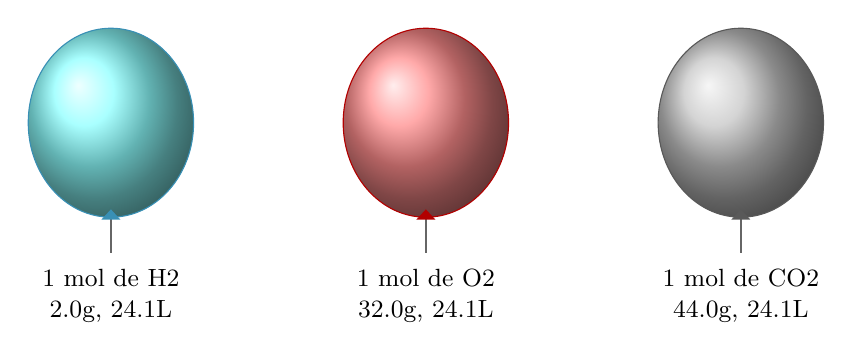
\begin{tikzpicture}[font=\small]
  \foreach \x/\g/\m/\c in {0/{\ce{H2}}/2.0/cyan, 4/{\ce{O2}}/32.0/red,
                           8/{\ce{CO2}}/44.0/gray} {
    \draw[thick, black!60] (\x,-0.25) -- (\x,-1.1);
    \shade[ball color=\c!45, draw=\c!70!black] (\x,0.55) ellipse (1.05 and 1.2);
    \fill[\c!70!black] (\x-0.12,-0.68) -- (\x+0.12,-0.68) -- (\x,-0.55) -- cycle;
    \node[align=center] at (\x,-1.65) {1 mol de \g\\ \qty{\m}{g},
      \qty{24.1}{L}};
  }
\end{tikzpicture}

{\small Tres globos a \qty{20}{\celsius}, cada uno con un \omterm{def:g10:the-mole:amount}{mol} de un gas
distinto. Los volúmenes son iguales; las masas, no.}
\end{omfigure}


\begin{example}[Un globo de dióxido de carbono]\label{ex:g10:the-mole:balloon}
% ledger: aw:C, aw:O
Un globo contiene \qty{2.4}{L} de dióxido de carbono a
\qty{20}{\celsius}. Su cantidad es
$n = \qty{2.4}{L} / \qty{24.1}{L/mol} = \qty{0.10}{mol}$,
y su masa, $m = \qty{0.10}{mol} \times \qty{44.0}{g/mol} =
\qty{4.4}{g}$. El mismo globo lleno de hidrógeno contendría los mismos
\qty{0.10}{mol}, pero solo \qty{0.20}{g} de gas.
\end{example}

\begin{remark}[Gases pesados y gases ligeros]\label{rem:g10:the-mole:heavy}
Como un litro de cualquier gas contiene la misma cantidad, la masa de un
litro de gas es proporcional a su \omterm{def:g10:the-mole:molar-mass}{masa molar}. El \omterm{def:g4:air-a-mixture-of-gases:air}{aire}, una \omterm{def:g6:pure-substances-and-mixtures:mixture}{mezcla} de
alrededor de cuatro quintas partes de nitrógeno (\qty{28.0}{g/mol}) y
una quinta parte de oxígeno (\qty{32.0}{g/mol}), se comporta como un gas
de \omterm{def:g10:the-mole:molar-mass}{masa molar} de unos \qty{29}{g/mol}. Un gas de \omterm{def:g10:the-mole:molar-mass}{masa molar} mayor, como
el dióxido de carbono (\qty{44.0}{g/mol}), es más denso que el \omterm{def:g4:air-a-mixture-of-gases:air}{aire} y se
acumula en el fondo de una bodega cerrada; un gas de \omterm{def:g10:the-mole:molar-mass}{masa molar} menor,
como el helio (\qty{4.0}{g/mol}), sube.
\end{remark}

\section{Ejercicios}

\begin{exercise}[$\star$]\label{exo:g10:the-mole:1}
Calcula las \omterm{def:g10:the-mole:molar-mass}{masas molares} del dioxígeno \ce{O2}, el dinitrógeno
\ce{N2}, el metano \ce{CH4}, el amoniaco \ce{NH3} y el dióxido de
carbono \ce{CO2}.
\end{exercise}

\begin{exercise}[$\star$]\label{exo:g10:the-mole:2}
¿Qué \omterm{def:g10:the-mole:amount}{cantidad de sustancia} hay en \qty{36.0}{g} de agua? ¿Y en
\qty{4.0}{g} de metano?
\end{exercise}

\begin{exercise}[$\star$]\label{exo:g10:the-mole:3}
¿Cuál es la masa de \qty{0.25}{mol} de cloruro de sodio \ce{NaCl}? ¿Y
la de \qty{2.0}{mol} de dióxido de carbono?
\end{exercise}

\begin{exercise}[$\star$]\label{exo:g10:the-mole:4}
¿Cuántas \omterm{def:g7:atoms-and-molecules:molecule}{moléculas} hay en \qty{0.50}{mol} de dioxígeno? ¿Qué cantidad
de hierro contiene \num{3.0e24} \omterm{def:g7:atoms-and-molecules:atom}{átomos} de hierro?
\end{exercise}

\begin{exercise}[$\star$]\label{exo:g10:the-mole:5}
A \qty{20}{\celsius} y a la presión atmosférica normal, ¿qué volumen
ocupan \qty{0.50}{mol} de dinitrógeno? ¿Qué cantidad de dioxígeno hay en
\qty{12}{L} de ese gas?
\end{exercise}

\begin{exercise}[$\star\star$]\label{exo:g10:the-mole:6}
Una gota de agua tiene un volumen de \qty{0.050}{mL}, y \qty{1}{mL} de
agua tiene una masa de \qty{1.0}{g}. ¿Cuántas \omterm{def:g7:atoms-and-molecules:molecule}{moléculas} de agua contiene
la gota?
\end{exercise}

\begin{exercise}[$\star\star$]\label{exo:g10:the-mole:7}
¿Qué contiene más \omterm{def:g7:atoms-and-molecules:atom}{átomos}, \qty{10}{g} de aluminio o \qty{10}{g} de
hierro? Explícalo primero sin calcular y compruébalo después
calculando.
\end{exercise}

\begin{exercise}[$\star\star$]\label{exo:g10:the-mole:8}
A \qty{20}{\celsius}, calcula la masa de un litro de dióxido de carbono
y la de un litro de dinitrógeno. ¿Por qué se acumula el dióxido de
carbono en el fondo de una bodega cerrada donde fermenta mosto?
\end{exercise}

\begin{exercise}[$\star\star$]\label{exo:g10:the-mole:9}
Con la figura de las tres cajas $m$, $n$, $N$, da la masa de
\num{1.0e22} \omterm{def:g7:atoms-and-molecules:molecule}{moléculas} de glucosa \ce{C6H12O6}. Indica las dos flechas
que has seguido.
\end{exercise}

\begin{exercise}[$\star\star$]\label{exo:g10:the-mole:10}
Un terrón de azúcar (sacarosa, \ce{C12H22O11}) tiene una masa de
\qty{5.0}{g}. Calcula la cantidad de sacarosa que contiene, después el
número de \omterm{def:g7:atoms-and-molecules:molecule}{moléculas} de sacarosa y, por último, el número de \omterm{def:g7:atoms-and-molecules:atom}{átomos} de
carbono.
\end{exercise}

\begin{exercise}[$\star\star$]\label{exo:g10:the-mole:11}
¿Qué contiene mayor cantidad de \omterm{def:g7:atoms-and-molecules:molecule}{moléculas}: \qty{1.0}{kg} de agua
\ce{H2O} o \qty{1.0}{kg} de etanol \ce{C2H6O}? ¿En qué factor?
\end{exercise}

\begin{exercise}[$\star\star\star$]\label{exo:g10:the-mole:12}
Un anillo de oro tiene una masa de \qty{5.0}{g}; tres cuartas partes de
su masa son oro, y el resto, cobre. ¿Cuántos \omterm{def:g7:atoms-and-molecules:atom}{átomos} de oro contiene?
¿Cuántos \omterm{def:g7:atoms-and-molecules:atom}{átomos} de cobre? ¿Qué \omterm{def:g9:periodic-table-first-look:metal}{metal} tiene más \omterm{def:g7:atoms-and-molecules:atom}{átomos} en el anillo?
\end{exercise}

\begin{exercise}[$\star\star\star$]\label{exo:g10:the-mole:13}
Un aula mide \qty{8.0}{m} por \qty{6.0}{m} por \qty{3.0}{m}, y el \omterm{def:g4:air-a-mixture-of-gases:air}{aire}
que contiene está a \qty{20}{\celsius}.
\begin{enumerate}
  \item ¿Qué cantidad de gas contiene ($\qty{1}{m^3} =
        \qty{1000}{L}$)? ¿Cuántas \omterm{def:g7:atoms-and-molecules:molecule}{moléculas}?
  \item Tomando el \omterm{def:g4:air-a-mixture-of-gases:air}{aire} como 78 \omterm{def:g7:atoms-and-molecules:molecule}{moléculas} de dinitrógeno, 21 de
        dioxígeno y 1 de argón (\qty{40.0}{g/mol}) de cada cien, calcula
        la \omterm{def:g10:the-mole:molar-mass}{masa molar} media del \omterm{def:g4:air-a-mixture-of-gases:air}{aire}.
  \item ¿Cuál es la masa del \omterm{def:g4:air-a-mixture-of-gases:air}{aire} del aula?
\end{enumerate}
\end{exercise}

\begin{exercise}[$\star\star\star$]\label{exo:g10:the-mole:14}
Una esfera de silicio puro tiene una masa de exactamente \qty{1.000}{kg}.
\begin{enumerate}
  \item ¿Cuántos \omterm{def:g7:atoms-and-molecules:atom}{átomos} de silicio contiene?
  \item Deduce la masa de un \omterm{def:g7:atoms-and-molecules:atom}{átomo} de silicio.
  \item Antes de 2019, la \omterm{def:g10:the-mole:avogadro}{constante de Avogadro} no estaba fijada, sino
        que se medía. Explica cómo un recuento independiente de los
        \omterm{def:g7:atoms-and-molecules:atom}{átomos} de una esfera así, cuya cantidad se conoce por su masa,
        daría un valor de ella.
\end{enumerate}
\end{exercise}

\begin{exercise}[$\star\star\star$]\label{exo:g10:the-mole:15}
% ledger: iso:Cl35, iso:Cl37
El cloro natural contiene un \qty{75.8}{\percent} de \omterm{def:g7:atoms-and-molecules:atom}{átomos} de cloro~35,
de \omterm{def:g10:the-mole:molar-mass}{masa molar} muy próxima a \qty{35.0}{g/mol}, y un \qty{24.2}{\percent}
de \omterm{def:g7:atoms-and-molecules:atom}{átomos} de cloro~37, de \omterm{def:g10:the-mole:molar-mass}{masa molar} muy próxima a \qty{37.0}{g/mol}.
Calcula la \omterm{def:g10:the-mole:molar-mass}{masa molar atómica} del cloro natural y compárala con el valor
de la tabla.
\end{exercise}

\section{Problema: El vaso de agua de Kelvin}

\begin{problem}[{Problema de fin de semana --- echa un vaso de agua al
mar, espera a que se mezcle por todos los océanos y vuelve a llenar un
vaso: ¿cuántas de las primeras moléculas vuelven?}]
\label{pb:g10:the-mole:1}
% ledger: ocean:volume, rho:water, const:NA, aw:H, aw:O
Un famoso experimento mental, atribuido a menudo al físico lord Kelvin,
dice así. Se marcan todas las \omterm{def:g7:atoms-and-molecules:molecule}{moléculas} de un vaso de agua, se vierte el
vaso en el mar y se espera a que las \omterm{def:g7:atoms-and-molecules:molecule}{moléculas} marcadas se hayan
repartido por igual por todos los océanos del mundo. Después se vuelve a
meter el vaso en el mar, en cualquier sitio. ¿Traerá alguna \omterm{def:g7:atoms-and-molecules:molecule}{molécula}
marcada? El vaso contiene \qty{250}{mL}, y \qty{1}{mL} de agua tiene una
masa de \qty{1.0}{g}. Los océanos contienen unos \qty{1.335e9}{km^3} de
agua. Para el recuento, trata el agua del mar como agua pura.

\medskip
\noindent\textbf{Parte I --- El agua de un vaso.}
\begin{enumerate}
  \item Calcula la \omterm{def:g10:the-mole:molar-mass}{masa molar} del agua.
  \item ¿Cuál es la masa del agua del vaso?
  \item Calcula la cantidad de \omterm{def:g7:atoms-and-molecules:molecule}{moléculas} de agua del vaso.
  \item ¿Qué cantidad de \omterm{def:g7:atoms-and-molecules:atom}{átomos} de hidrógeno contiene el vaso? ¿Y de
        \omterm{def:g7:atoms-and-molecules:atom}{átomos} de oxígeno?
\end{enumerate}

\medskip
\noindent\textbf{Parte II --- Las \omterm{def:g7:atoms-and-molecules:molecule}{moléculas} del vaso.}
\begin{enumerate}[resume]
  \item ¿Cuántas \omterm{def:g7:atoms-and-molecules:molecule}{moléculas} de agua contiene el vaso?
  \item Calcula la masa de una \omterm{def:g7:atoms-and-molecules:molecule}{molécula} de agua, en gramos.
  \item Comprueba las respuestas a las preguntas 5 y 6 multiplicándolas:
        ¿cuánto debería dar el producto?
  \item Contando una \omterm{def:g7:atoms-and-molecules:molecule}{molécula} por segundo, día y noche, ¿cuántos años
        harían falta para contar las \omterm{def:g7:atoms-and-molecules:molecule}{moléculas} del vaso? (Un año dura
        unos \qty{3.16e7}{s}.)
\end{enumerate}

\medskip
\noindent\textbf{Parte III --- El océano.}
\begin{enumerate}[resume]
  \item Pasa el volumen de los océanos a metros cúbicos
        ($\qty{1}{km^3} = \qty{e9}{m^3}$) y después a litros.
  \item Una vez repartidas por igual las \omterm{def:g7:atoms-and-molecules:molecule}{moléculas} marcadas, ¿cuántas
        hay en cada litro de océano?
  \item ¿Cuántas \omterm{def:g7:atoms-and-molecules:molecule}{moléculas} marcadas trae el segundo vaso?
  \item Segundo método. Calcula la cantidad de agua de los océanos,
        tomando \qty{1.0}{kg} como masa de un litro.
  \item ¿Qué fracción de todas las \omterm{def:g7:atoms-and-molecules:molecule}{moléculas} de agua del océano están
        marcadas?
  \item Multiplica esta fracción por el número de \omterm{def:g7:atoms-and-molecules:molecule}{moléculas} del segundo
        vaso, y compáralo con la respuesta a la pregunta 11.
\end{enumerate}

\medskip
\noindent\textbf{Parte IV --- Lo que significa.}
\begin{enumerate}[resume]
  \item ¿Cuántos vasos de \qty{250}{mL} se podrían llenar con el agua de
        los océanos?
  \item Compara este número con el número de \omterm{def:g7:atoms-and-molecules:molecule}{moléculas} de un vaso.
        Explica en una frase por qué el segundo vaso trae tantas
        \omterm{def:g7:atoms-and-molecules:molecule}{moléculas} marcadas.
  \item ¿Qué volumen de agua de mar hay que sacar, por término medio,
        para recuperar una sola \omterm{def:g7:atoms-and-molecules:molecule}{molécula} marcada? Compáralo con una gota
        de \qty{0.05}{mL}.
  \item La respuesta a la pregunta 11 tiene muchas cifras. ¿Por qué solo
        hay que darla como orden de magnitud? Da dos razones.
  \item Da la respuesta final: ¿cuántas \omterm{def:g7:atoms-and-molecules:molecule}{moléculas}, más o menos, del
        primer vaso vuelven en el segundo?
\end{enumerate}
\end{problem}
